\chapter{Many fiber simulations} \label{chap:four}

	\begin{figure}
		\begin{center}
			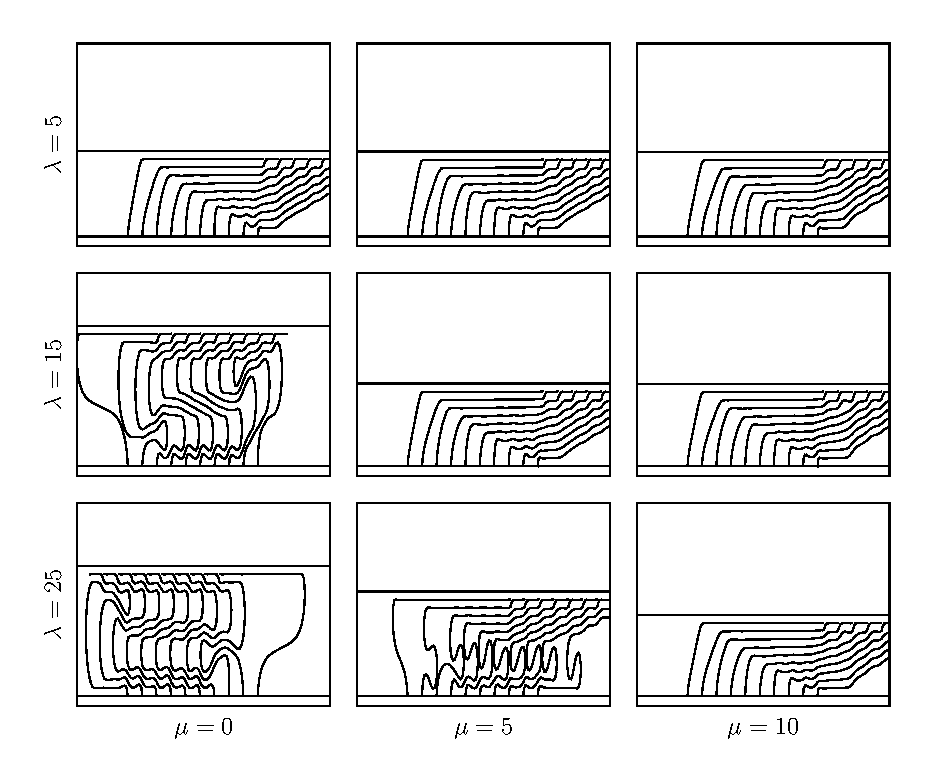
\includegraphics[scale=1]{./fig/ch4/grid.eps}
		\end{center}		
		\caption{Phase plot of a fiber's torsional spring strength, $\beta$, against the strength of the bottom substrate's vdW force, $\eps^-$.
		\label{fig:grid}}
	\end{figure}

	\begin{figure}
		\begin{center}
			\includegraphics[scale=1]{./fig/ch4/grid_b100.eps}
		\end{center}		
		\caption{Phase plot of a fiber's torsional spring strength, $\beta$, against the strength of the bottom substrate's vdW force, $\eps^-$.
		\label{fig:grid_b100}}
	\end{figure}
	
	\begin{figure}
		\begin{center}
			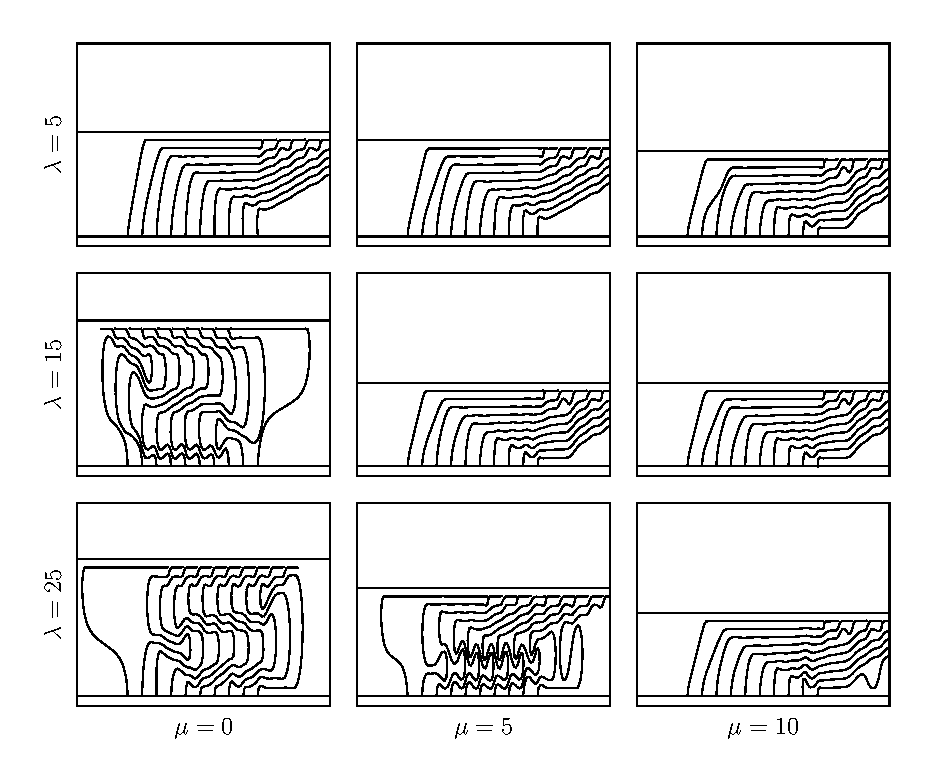
\includegraphics[scale=1]{./fig/ch4/grid_g1000.eps}
		\end{center}		
		\caption{Phase plot of a fiber's torsional spring strength, $\beta$, against the strength of the bottom substrate's vdW force, $\eps^-$.
		\label{fig:grid_g1000}}
	\end{figure}
	
	\begin{figure}
		\begin{center}
			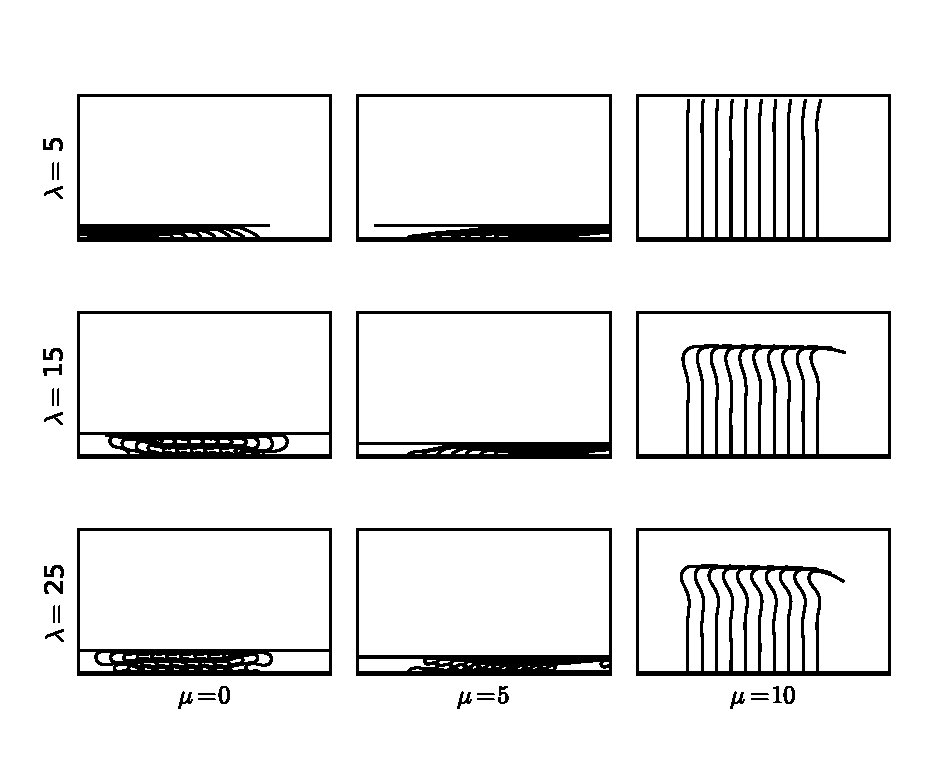
\includegraphics[scale=1]{./fig/ch4/grid_et0.1.eps}
		\end{center}		
		\caption{Phase plot of a fiber's torsional spring strength, $\beta$, against the strength of the bottom substrate's vdW force, $\eps^-$.
		\label{fig:grid_et0.1}}
	\end{figure}

Similar to a single fiber case, the moving substrate is pushed into the forest, compressing the fibers until an equilibrium is reached. This force is then relaxed. A similar set of case studies are then applied to the many fiber case in order to find the minimum necessary magnitude to pull off the moving substrate.